\chapter{Modellazione e sviluppo dell'ontologia}

L'ontologia è stata creata partendo da una focalizzazione sulle entità primarie.

\section{Prosumer}
Il prosumer è l'entità principale dell'ontologia, ciò che andrà a contenere le entità caratterizzanti.


\begin{figure}[!ht]
    \centering
    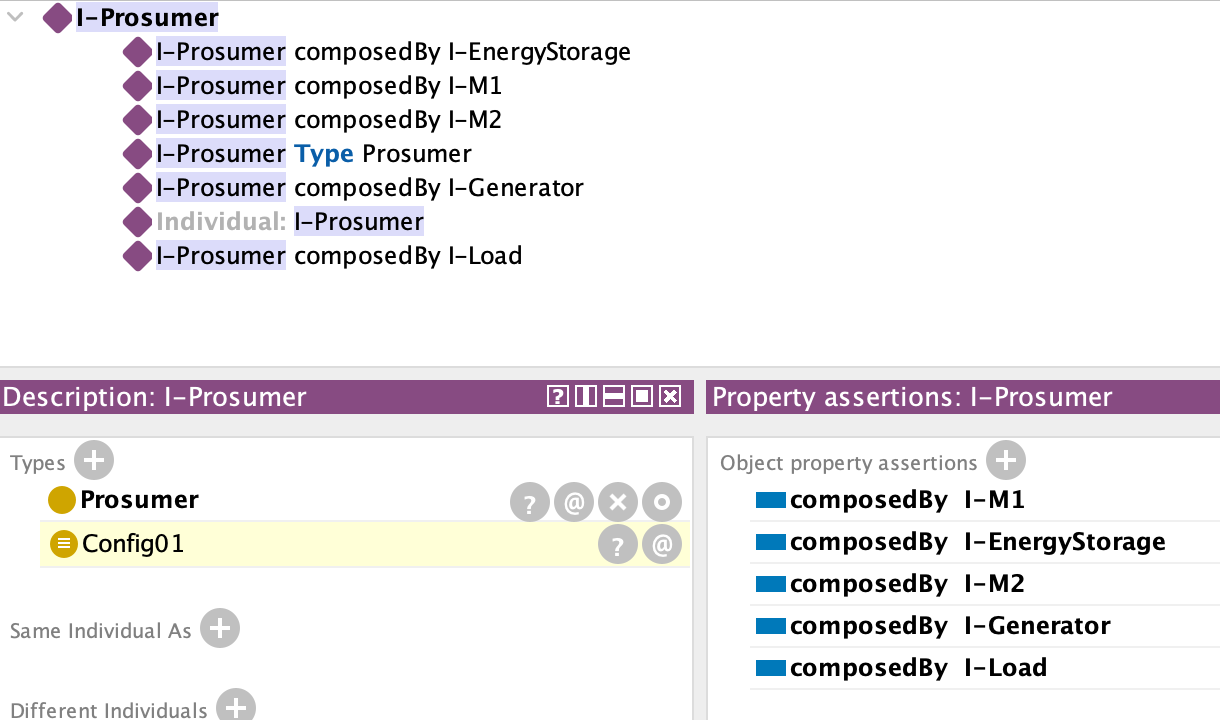
\includegraphics[width=12cm]{images/individual_prosumer.png}
    \caption{Prosumer applicato a un individuo su Protègè.}
    \label{fig:individual_prosumer}
\end{figure}

Come si può notare nell'immagine \ref*{fig:individual_prosumer}, al prosumer vengono assegnati altri individui tramite le proprietà, grazie a ciò il reasoner è in grado di inferire la tipologia di configurazione.
In questo caso è di tipo Config01, siccome Energy Storage rispetta le caratteristiche della configurazione, come verrà mostrato nelle sezioni successive.

\subsection{Configuration}
Per stabilire la tipologia di configurazione, è stata creata la sottoclasse Configuration che a sua volta possiede le sottoclassi Config01, Config02 e Config03.

\begin{figure}[!ht]
    \centering
    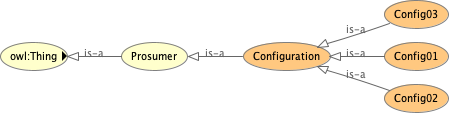
\includegraphics[width=12cm]{images/pros_graph.png}
    \caption{Grafico creato su Protègè tramite il plugin OWLViz.}
    \label{fig:pros_graph}
\end{figure}

Per specificare le caratteristiche di ogni configurazione, sono state espresse le condizioni necessarie e sufficienti. Per ogni configurazione sono presenti:
\begin{verbatim}
    Prosumer 
     and (composedBy some Generator) 
     and (composedBy some Load) 
     and (composedBy some M1) 
     and (composedBy some M2) 
\end{verbatim}

Mentre, in aggiunta per ogni configurazione:
\begin{itemize}
    \item Configurazione 01: condizioni necessarie e sufficienti: \begin{verbatim}
        and (composedBy some 
            (StorageSystem 
             and (hasDirection some Monodirectional) 
             and (hasLocation some Production) 
             and (hasPowerType some DC)))
    \end{verbatim}
          condizioni necessarie: \begin{verbatim}
        Prosumer and (not (composedBy some M3))
    \end{verbatim}
    \item Configurazione 02: condizioni necessarie e sufficienti: \begin{verbatim}
        and (composedBy some 
            (StorageSystem 
             and (hasDirection some Bidirectional) 
             and (hasLocation some Production) 
             and (hasPowerType some (AC or DC))))
    \end{verbatim}
          condizioni necessarie: \begin{verbatim}
        Prosumer and (not (composedBy some M3))
    \end{verbatim}
    \item Configurazione 03: condizioni necessarie e sufficienti \begin{verbatim}
         and (composedBy some M3) 
         and (composedBy some 
            (StorageSystem 
             and (hasDirection some Bidirectional) 
             and (hasLocation some Post-Production)
             and (hasPowerType some AC)))
    \end{verbatim}
\end{itemize}


\section{Generator}
IL generatore rappresenta l'entità che produce energia ed è presente in tutti i prosumer.
L'energia prodotta dal generatore servirà a soddisfare il Load, a caricare lo Storage System e quella in eccesso verrà immessa nella rete.
\begin{figure}[H]
    \centering
    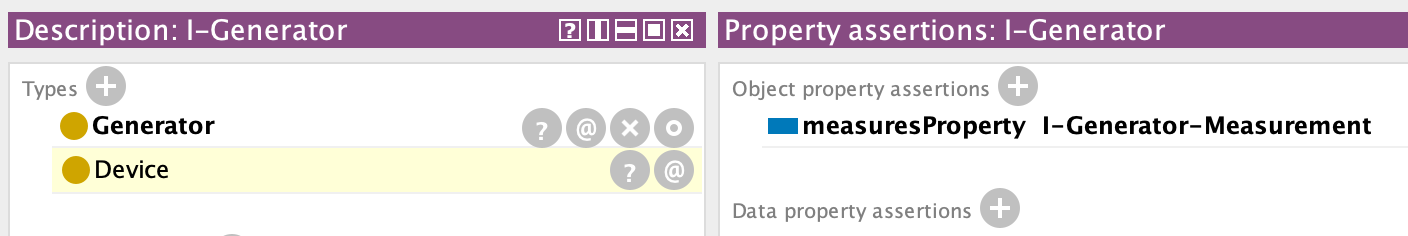
\includegraphics[width=12cm]{images/individual_generator.png}
    \caption{Istanza di un individuo di tipo generatore.}
    \label{fig:individual_generator}
\end{figure}

Per monitorare l'energia prodotta dal generatore, è stata definita un'istanza della classe "Time Series" (figura \ref{fig:individual_genmeas}), importata dall'ontologia ic-data. In questo modo si può definire un intervallo temporale e creare una sequenza di "Data Point"(anch'essa classe importata da ic-data), uno per ogni intervallo di tempo.
\begin{figure}[H]
    \centering
    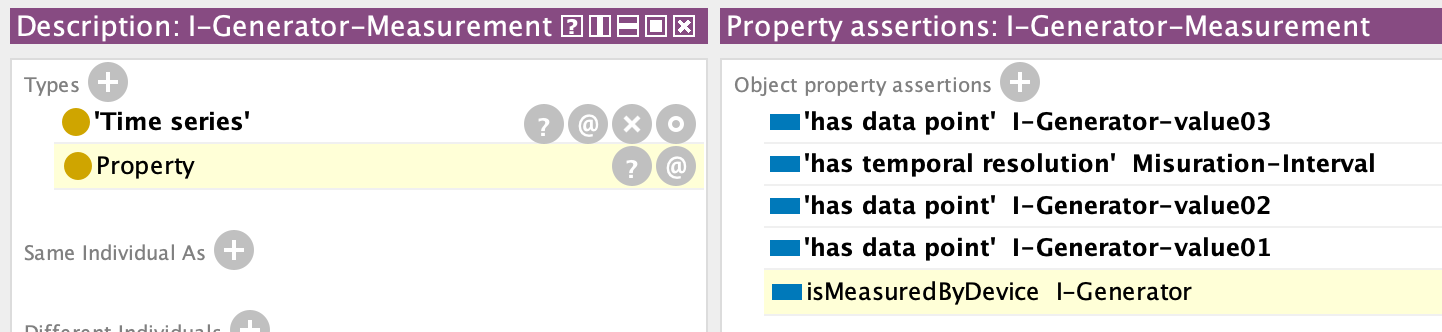
\includegraphics[width=12cm]{images/individual_genmeas.png}
    \caption{Istanza di un individuo di tipo Time Series per il generatore.}
    \label{fig:individual_genmeas}
\end{figure}
Ogni singolo "GeneratorMeasurement" è quindi sottoclasse di Data Point e rappresenta un'osservazione dell'energia prodotta dal generatore in un intervallo di tempo specificato dal timestamp (figura \ref{fig:individual_genval3}).
\begin{figure}[H]
    \centering
    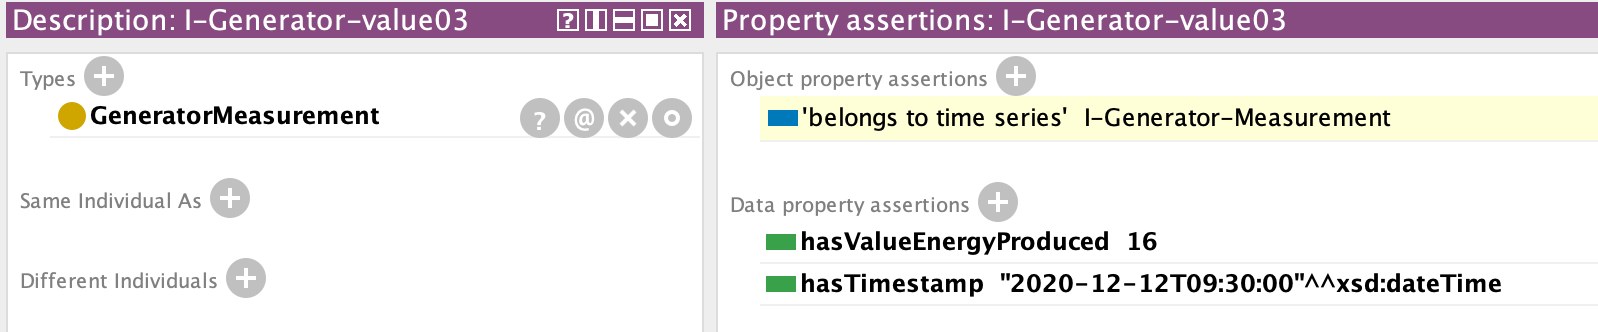
\includegraphics[width=12cm]{images/individual_genval3.png}
    \caption{Istanza di un individuo di tipo GeneratorMeasurement.}
    \label{fig:individual_genval3}
\end{figure}


\section{Load}
Il Load rappresenta il profilo di carico equivalente, anche detto consumo, del prosumer.
\begin{figure}[H]
    \centering
    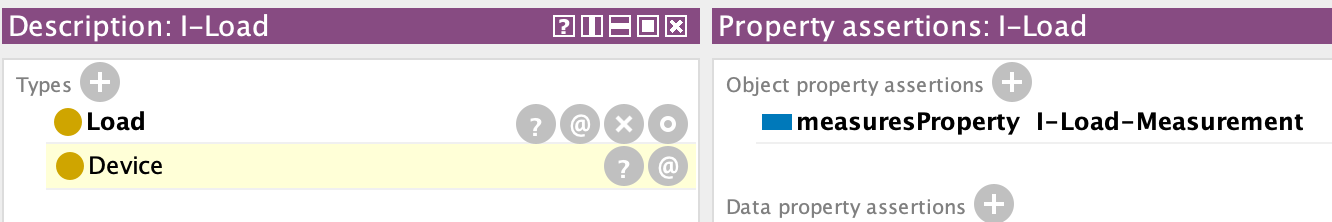
\includegraphics[width=12cm]{images/individual_load.png}
    \caption{Istanza di un individuo di tipo Load.}
    \label{fig:individual_load}
\end{figure}
Analogamente per quanto fatto per il generatore, anche per il Load è stata definita un'istanza della classe "Time Series" (figura \ref{fig:individual_loadmes}) e ogni singolo "LoadMeasurement"
è sottoclasse di Data Point (figura \ref{fig:individual_loadval3}).
\begin{figure}[H]
    \centering
    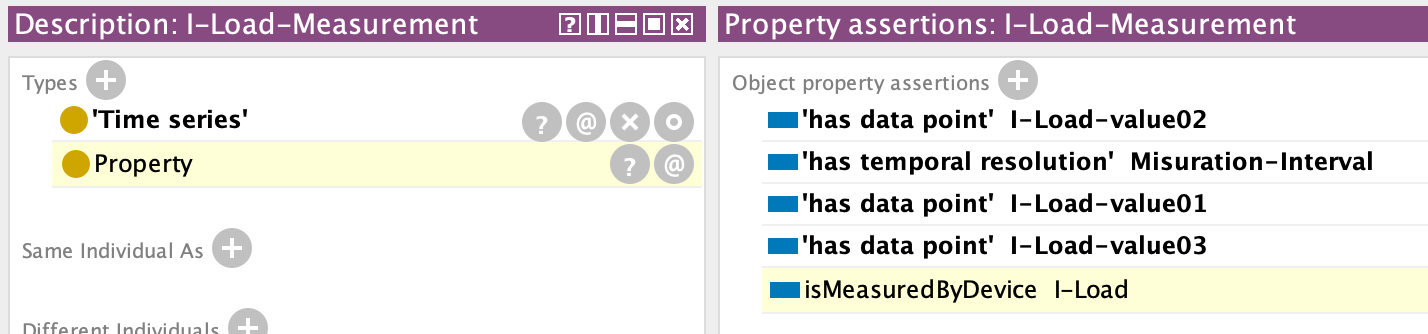
\includegraphics[width=12cm]{images/individual_loadmes.png}
    \caption{Istanza di un individuo di tipo Time Series per il Load.}
    \label{fig:individual_loadmes}
\end{figure}
In questo modo si va a specificare l'energia consumata dal prosumer in un intervallo di tempo specificato dal timestamp, fornendo una visione dettagliata dell'utilizzo dell'energia da parte del prosumer nel corso del tempo.
\begin{figure}[H]
    \centering
    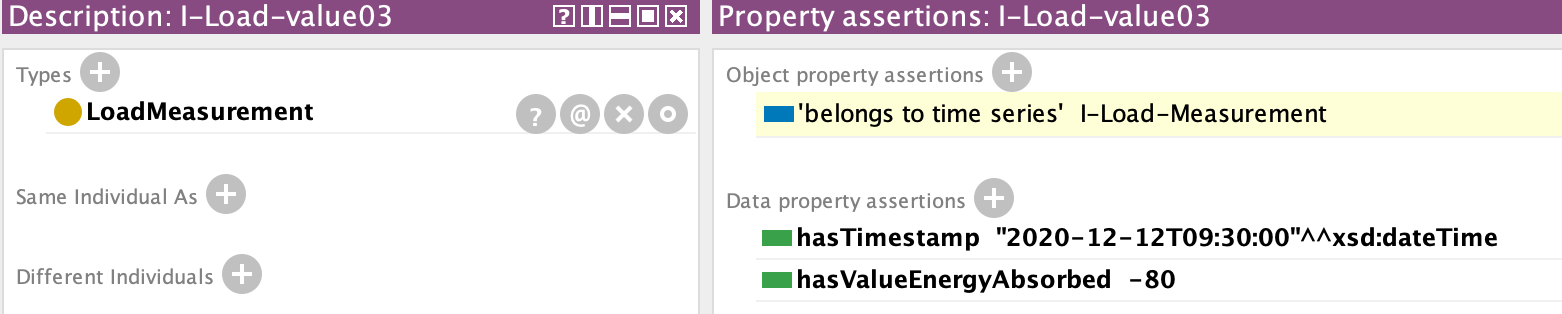
\includegraphics[width=12cm]{images/individual_loadval3.png}
    \caption{Istanza di un individuo di tipo LoadMeasurement.}
    \label{fig:individual_loadval3}
\end{figure}

\section{Storage System}
Lo Storage System è l'entità che rappresenta il sistema di accumulo dell'energia di un prosumer. Viene utilizzato per immagazzinare l'energia ed eventualmente per fornirla al prosumer in caso di necessità.
In questo caso è stata estesa l'ontologia \textit{Battery} sviluppata da Kyrillos, aggiungendo informazioni quali il tipo di corrente (AC o DC), la direzione del flusso energetico (monodirezionale o bidirezionale) e il posizionamento (produzione o post-produzione), utili per identificare la configurazione del prosumer.
In figura \ref{fig:individual_storagesystem} viene mostrata l'istanza di una classe StorageSystem, composto da due batterie, il tipo di corrente, la direzione del flusso e il posizionamento.
\begin{figure}[H]
    \centering
    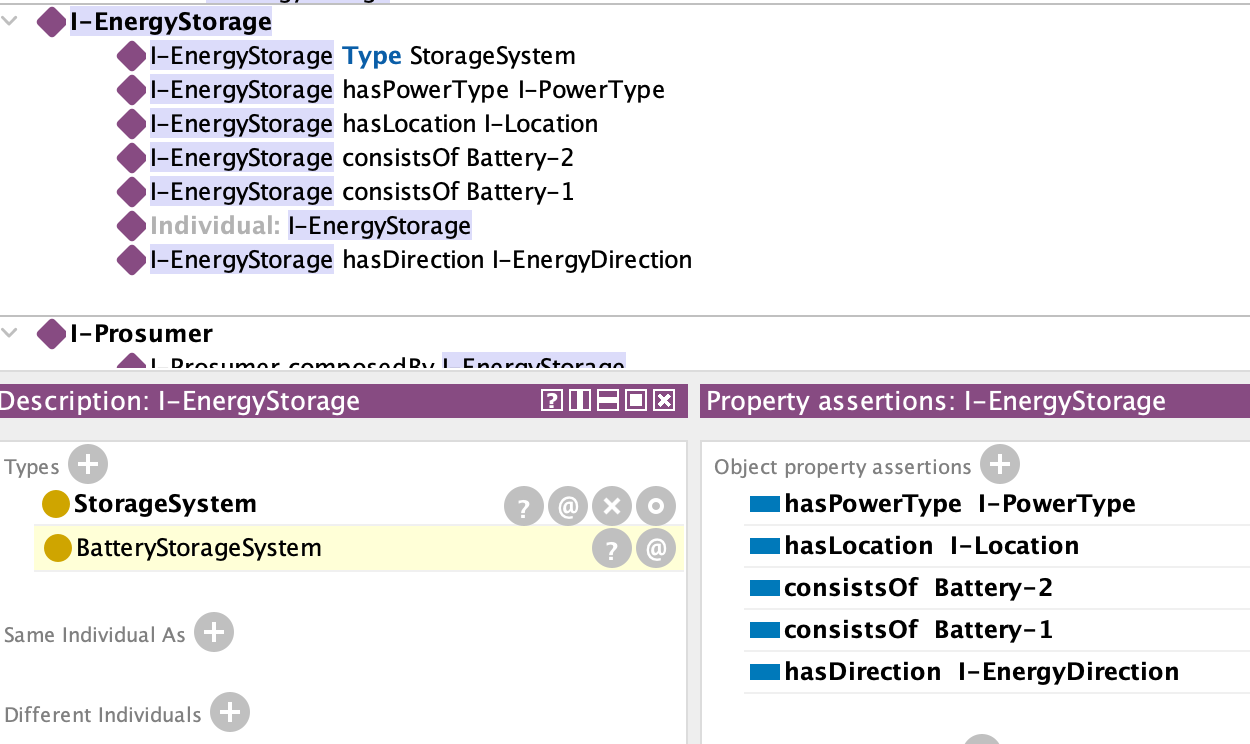
\includegraphics[width=12cm]{images/individual_storagesystem.png}
    \caption{Istanza di un individuo di tipo StorageSystem.}
    \label{fig:individual_storagesystem}
\end{figure}
Nella figura \ref{fig:individual_bat1} viene mostrata l'istanza di una classe Battery, in questo caso la Batteria 1 facente parte dello Storage System. Questa classe è utile per specificare le caratteristiche della batteria, salvate come Data Property.
\begin{figure}[H]
    \centering
    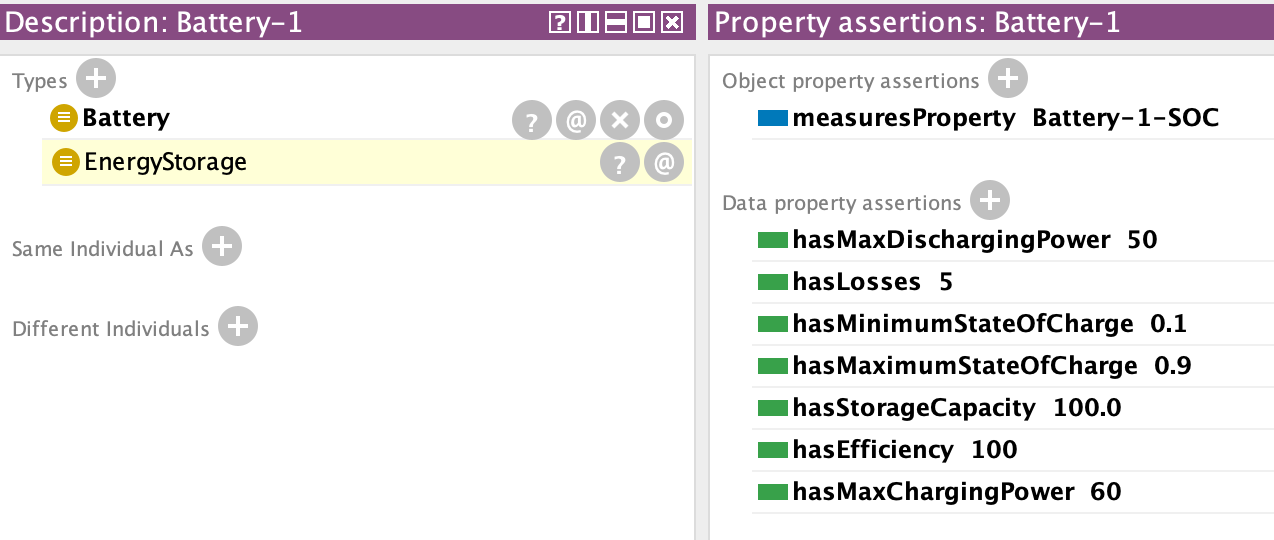
\includegraphics[width=12cm]{images/individual_bat1.png}
    \caption{Istanza di un individuo di tipo Battery.}
    \label{fig:individual_bat1}
\end{figure}
La classe StateOfCharge è sottoclasse di Time Series, quindi la sua utilità è quella di avere il riferimento a una sequenza di misurazioni.
\begin{figure}[H]
    \centering
    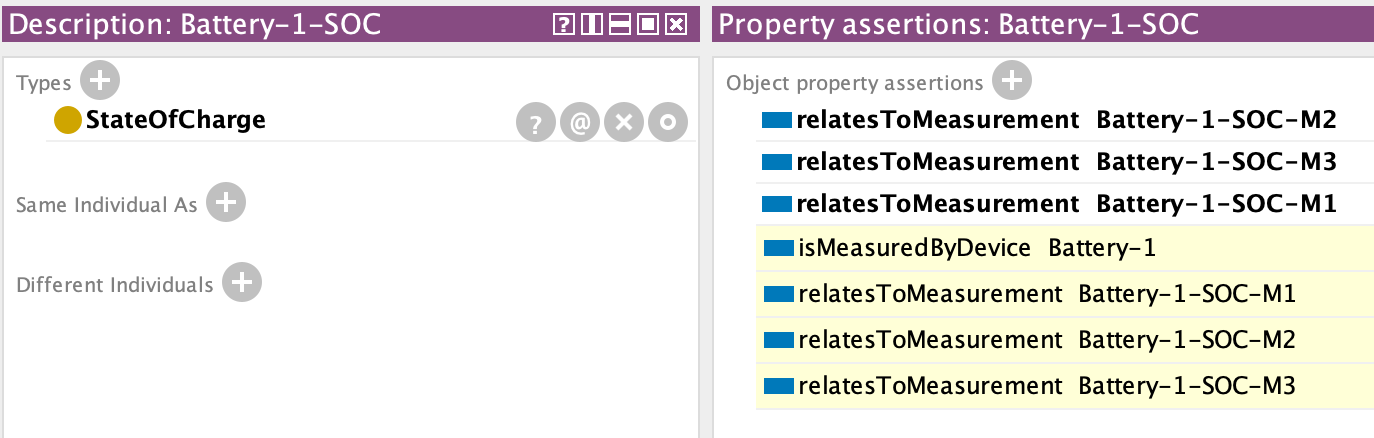
\includegraphics[width=12cm]{images/individual-batterysoc.png}
    \caption{Istanza di un individuo di tipo StateOfCharge.}
    \label{fig:individual-batterysoc}
\end{figure}
Ogni misurazione è rappresentata da un'istanza di StateOfChargeMeasurement, sottoclasse di Data Point.
In figura \ref{fig:individual_batterym3} si possono notare le due Data Property inferite grazie alle regole SWRL descritte nella sezione \ref{sec:swrl}.
\begin{figure}[H]
    \centering
    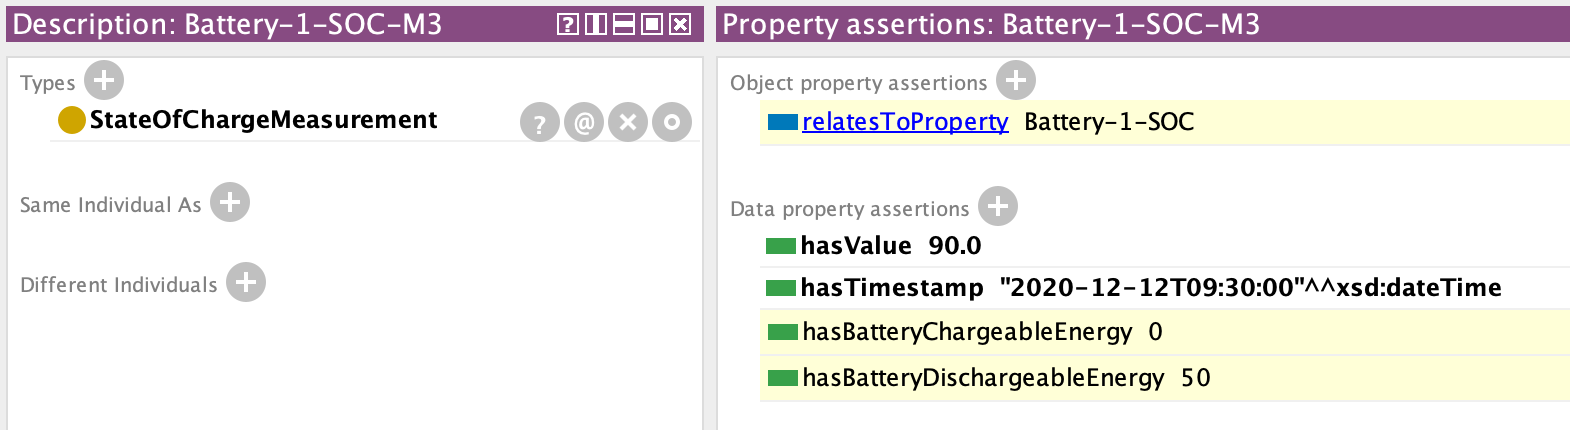
\includegraphics[width=12cm]{images/individual-batterym3.png}
    \caption{Istanza di un individuo di tipo StateOfChargeMeasurement.}
    \label{fig:individual_batterym3}
\end{figure}

\section{Energy Meter}
L'Energy Meter è l'entità che rappresenta il contatore di energia di un prosumer. Come già descritto nella sezione \ref{sec:analisi_dominio} un prosumer deve avere un contatore di tipo M1, un contatore di tipo M2 e, solo per la configurazione tre, un contatore di tipo M3.
Questi tre tipi di contatori sono stati rappresentati con tre classi distinte, definite come sottoclassi della classe EnergyMeter.

In figura \ref{fig:individual_m1} viene mostrata l'istanza di una classe M1, in questo caso il contatore M1 facente parte del prosumer.
\begin{figure}[H]
    \centering
    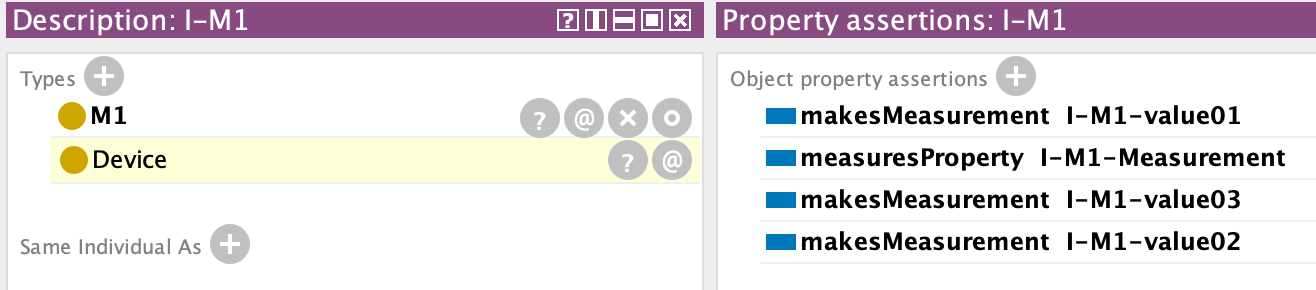
\includegraphics[width=12cm]{images/individual_m1.png}
    \caption{Istanza di un individuo di tipo M1.}
    \label{fig:individual_m1}
\end{figure}

Come per gli altri componenti, anche il contatore ha una sequenza di misurazioni, rappresentata dalla classe Time Series.

\begin{figure}[H]
    \centering
    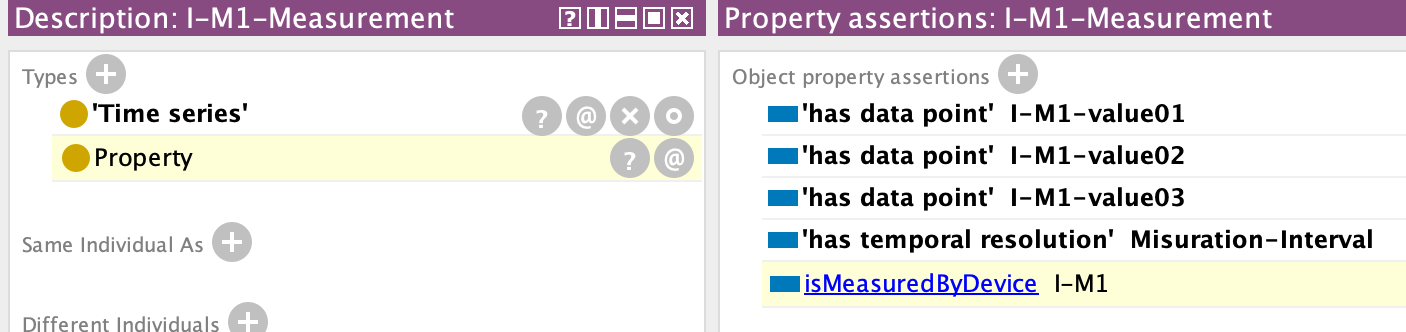
\includegraphics[width=12cm]{images/individual_m1meas.png}
    \caption{Istanza di un individuo di tipo Time Series per M1.}
    \label{fig:individual_m1meas}
\end{figure}

Ogni misurazione è rappresentata da un'istanza di EnergyMeterMeasurement, sottoclasse di Data Point. Si può notare dalla figura \ref{fig:individual_m1val3} che nel caso dei contatori nella misurazione è stato inserito solo il valore del timestamp, in quanto il valore dell'energia scambiata è calcolato con le query SPARQL descritte nella sezione \ref{sec:sparql}.

\begin{figure}[H]
    \centering
    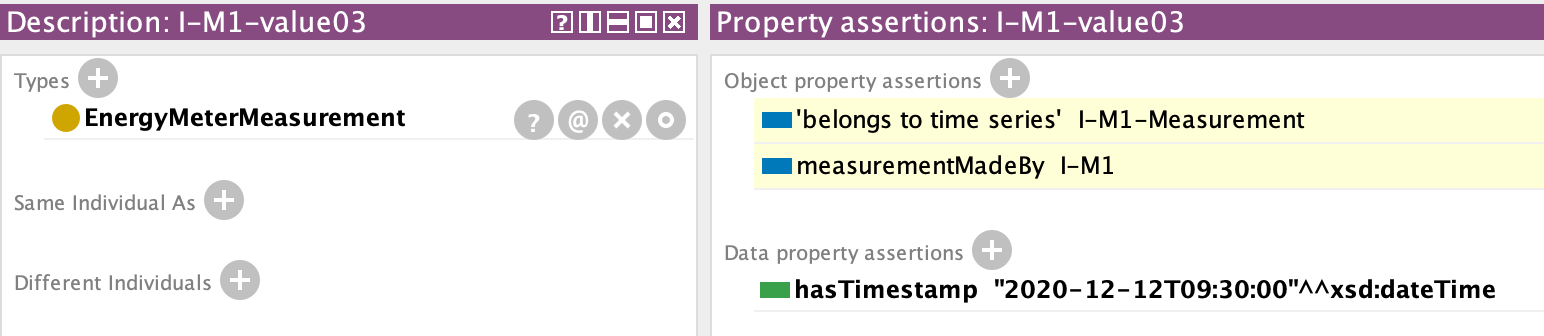
\includegraphics[width=12cm]{images/individual_m1val3.png}
    \caption{Istanza di un individuo di tipo EnergyMeterMeasurement}
    \label{fig:individual_m1val3}
\end{figure}